\documentclass[
	a4paper,			% Paper size, refrain from changing this                
	11pt,				% Font size, change to your liking,
						% standard size is 11 for a thesis.
	headsepline,		% Shows a separation line between section,
						% or chapter name and the actual text.
	bibtotoc,			% Shows that a bibliography exists in the table
						% of contents.
	BCOR18mm,      		% Enables left/right spacing for the 
						% glue-binding,
						% if only one-sided print no right spacing.				
	DIV14,				% Ignore these
	headings=normal,
	numbers=noenddot,
]{scrbook}

%%%%%%%%%%%%%%%%%%%%%%%%%%%%%%%%%%%%%%%%%%%%%%%%%%%%%%%%%%%%%%%%%%%%%%%%%%%%%%%%%
% Put new commands and other stuff in the preamble here,						%
% this may include abbreviations theorems or package loading.					%
% Some usual stuff is added here. 												%
% Examples can be found at the respective subpreamble point.					%
% For packages not needed it is suggested to just uncomment them.				%
%%%%%%%%%%%%%%%%%%%%%%%%%%%%%%%%%%%%%%%%%%%%%%%%%%%%%%%%%%%%%%%%%%%%%%%%%%%%%%%%%

% General useful to have
\usepackage[utf8]{inputenc}			% Sets encoding in *File* as UTF-8
\usepackage{enumerate}				% Enables <enumerate> environment, an 
\usepackage{subcaption}									% extension to the predefined one.
\usepackage{longtable}				% Enables <longtable> environment, hugely
\usepackage{pgfplots}
\usetikzlibrary{decorations.markings}
\pgfplotsset{compat=1.13}									% superior to tabular
\usepackage{hyperref}				% Make links, sections clickable
\usepackage{theoremref}				% And theorems clickable
\usepackage{setspace}				% Enables setting the spacing between lines
\usepackage{todonotes}				% Very useful tool for marking unfinished 
									% places
\usepackage{breakcites}				% Breaks citations in lines
\usepackage[splitrule]{footmisc}	% Draws a line above footnotes in a page
\interfootnotelinepenalty=10000 	% Completely prevent breaking of footnotes
\usepackage{tikz}					% Enable tikzpictures
\usetikzlibrary{decorations.pathreplacing,angles,quotes}
% Math
\usepackage{amsfonts}	% Enables mathscr font
\usepackage{amsmath}	% Enables general math commands
\usepackage{amssymb}	% Enables mathbb fonts (e.g. natural numbers symbol)
\usepackage{amsthm}		% Enables pre- and userdefined theorem environments
\usepackage{dsfont}		% Enables more fonts for numbers in math environment
\usetikzlibrary{calc}
% Glossary
\usepackage[toc,		% Add glossary entry to table of contents
			acronym,	% With abbreviations enabled
			automake]	% Makes life easier
{glossaries}
\makeglossaries			% Creates glossary
\newacronym{LatexMacroShorthand}{ShorthandSubstitution}{ShorthandDescription}
\newcommand\ellipsebyfoci[4]{% options, focus pt1, focus pt2, cste
  \path[#1] let \p1=(#2), \p2=(#3), \p3=($(\p1)!.5!(\p2)$)
  in \pgfextra{
    \pgfmathsetmacro{\angle}{atan2(\y2-\y1,\x2-\x1)}
    \pgfmathsetmacro{\focal}{veclen(\x2-\x1,\y2-\y1)/2/1cm}
    \pgfmathsetmacro{\lentotcm}{\focal*2*#4}
    \pgfmathsetmacro{\axeone}{(\lentotcm - 2 * \focal)/2+\focal}
    \pgfmathsetmacro{\axetwo}{sqrt((\lentotcm/2)*(\lentotcm/2)-\focal*\focal}
  }
  (\p3) ellipse[x radius=\axeone cm,y radius=\axetwo cm, rotate=\angle];
}
% Algorithm
\usepackage[ruled, 			% Enable vertical lines for for-loops / if's
			linesnumbered]	% Enable line numbering
{algorithm2e}
\newenvironment{myalgorithm}[1][htb]	% Set up user-defined algorithm 
										% environment
{
	% Set up a no-line command to disable line numbering
	\let\oldnl\nl
	\newcommand{\nonl}{\renewcommand{\nl}{\let\nl\oldnl}}
	
	\DontPrintSemicolon
	\SetAlgoVlined
	\SetArgSty{normalfont}
	\SetKwInOut{Input}{Input}
	\SetKwInOut{Output}{Output}
	\SetKw{Continue}{continue}
	\SetKwFor{ParForEach}{par foreach}{}{}
	\SetKw{Sequentially}{sequentially}
	\renewcommand{\algorithmcfname}{Algorithm}% Update algorithm name
	\begin{algorithm}[#1]%
	}{\end{algorithm}}

%%%%%%%%%%%%%%%%%%%%%%%%%%%%%%%%%%%%%%%%%%%%%%%%%%%%%%%%%%%%%%%%%%%%%%%%%%%%%%%%%
% Customization should be put here, enables customizing captions of figures,	%
% declaring math operators, custom colors etc.									%
%%%%%%%%%%%%%%%%%%%%%%%%%%%%%%%%%%%%%%%%%%%%%%%%%%%%%%%%%%%%%%%%%%%%%%%%%%%%%%%%%

% Setting the caption font of figures, in this example it will be set to a bold
% font with normalsize 
\usepackage[labelfont={bf,normalsize}]{caption}

% Setting automatically determined section headnames, this is required for the
% \autoref{...} command
\renewcommand{\chapterautorefname}{Chapter}
\renewcommand{\subsectionautorefname}{Subsection}
\renewcommand{\sectionautorefname}{Section}

% Set up custom theorem style, here bold.
% Additionally set up auto-reference names,
% to enable a homogenous numbering for either propositions, lemmas, theorems,
% etc we need to derive other styles from the first.
\usepackage{aliascnt}
\usepackage{fancyvrb}
\newtheoremstyle{mythmstyle}
{.75em} 		% Space above
{.75em} 		% Space below
{\normalfont}	% Body font
{} 				% Indent amount
{\bfseries} 	% Theorem head font
{.} 			% Punctuation after theorem head
{.75em} 		% Space after theorem head
{} 				% Theorem head spec (can be left empty, meaning `normal')
\theoremstyle{mythmstyle}

% First
\newtheorem{mylem}{Lemma}[chapter]

\newtheoremstyle{other}
{.75em} 		% Space above
{.75em} 		% Space below
{\normalfont} 	% Body font
{} 				% Indent amount
{\bfseries} 	% Theorem head font
{.} 			% Punctuation after theorem head
{.75em} 		% Space after theorem head
{} 				% Theorem head spec (can be left empty, meaning `normal')
\theoremstyle{other}

% Derivations

% Definition
\newaliascnt{mydef}{mylem}
\newtheorem{mydef}[mydef]{Definition}
\aliascntresetthe{mydef}
\providecommand*{\mydefautorefname}{Definition}
% Theorem
\newaliascnt{mythm}{mylem}
\newtheorem{mythm}[mythm]{Theorem}
\aliascntresetthe{mythm}
\providecommand*{\mythmautorefname}{Theorem}
% Notation
\newaliascnt{mynot}{mylem}
\newtheorem{mynot}[mynot]{Notation}
\aliascntresetthe{mynot}
\providecommand*{\mynotautorefname}{Notation}
% Example
\newaliascnt{myexp}{mylem}
\newtheorem{myexp}[myexp]{Example}
\aliascntresetthe{myexp}
\providecommand*{\myexpautorefname}{Example}
% Proposition
\newaliascnt{myprop}{mylem}
\newtheorem{myprop}[myprop]{Proposition}
\aliascntresetthe{myprop}
\providecommand*{\mypropautorefname}{Proposition}
% Corollary
\newaliascnt{mycor}{mylem}
\newtheorem{mycor}[mycor]{Corollary}
\aliascntresetthe{mycor}
\providecommand*{\mycorautorefname}{Corollary}
% Remark
\newaliascnt{myrem}{mylem}
\newtheorem{myrem}[myrem]{Remark}
\aliascntresetthe{myrem}
\providecommand*{\myremautorefname}{Remark}
% Heuristic
\newaliascnt{myheu}{mylem}
\newtheorem{myheu}[myheu]{Heuristic}
\aliascntresetthe{myheu}
\providecommand*{\myheuautorefname}{Heuristic}

% Provide more autoref changes
\renewcommand{\tableautorefname}{Table}
\renewcommand{\figureautorefname}{Figure}
\renewcommand{\sectionautorefname}{Section}
\newcommand{\mylemautorefname}{Lemma}

% Set indentation of new paragraph
\setlength\parindent{15pt}

% Allow math environments to break to new line
\allowdisplaybreaks

% Change to line spacing between lines
\renewcommand{\baselinestretch}{1.2}

% Prevent math designated formulas to go beyond text
\allowbreak

% Further border settings
\typearea[20mm]{15}

% Set language for bibliography etc, most likely british, USamerican or german
\usepackage[british]{babel}

% Show dots connecting sections and number in table of contents
\usepackage{tocloft}
\renewcommand{\cftsecleader}{\cftdotfill{\cftdotsep}}

% Enable equation numbering
\renewcommand{\theequation}{\thechapter.\arabic{equation}}

%%%%%%%%%%%%%%%%%%%%%%%%%%%%%%%%%%%%%%%%%%%%%%%%%%%%%%%%%%%%%%%%%%%%%%%%%%%%%%%%%
% Title Page Layout 															%
%%%%%%%%%%%%%%%%%%%%%%%%%%%%%%%%%%%%%%%%%%%%%%%%%%%%%%%%%%%%%%%%%%%%%%%%%%%%%%%%%
% Angaben für das Titelblatt
\titlehead{
	\begin{flushright}
		
\includegraphics[scale=0.2]{Goethe-Logo-blau}
		\vspace{1cm}
	\end{flushright}
}
% Art der Arbeit
\subject{Bachelorarbeit}
% Titel
\title{Modellierung der Elektrophysiologie des Herzens}

\author{Julian Lucas Hilbert \\
		Studiengang: B.Sc. Informatik\\
		Matrikelnummer: 5533406}

% Adjust language if needed
\publishers{
	\normalsize
	
	\vspace{0.3cm}
	{
	\begin{tabular}{l l}
		Examiner: & <Examiner>\\
		Advisor: & <Advisor>
	\end{tabular}\\
	}
	\vspace{0.5cm}
	
	Professorship for <Working Group>\\
	Institute of Computer Science\\
	Department of Computer Science and Mathematics\\
	Goethe University Frankfurt
	\vspace{-2cm}
}

% Set date
\date{ \vspace{2cm} Frankfurt am Main \\ xx.xx.2018}

\begin{document}
{
	% Set table of contents depth to only chapters and sections, increase to 
	% show subsections or even subsubsections, lower for only chapters
	\setcounter{tocdepth}{1}
	
	% Ignore this, necessary for the title page and numbering issues
	\pagestyle{empty}
	\maketitle
	
	% Put your thanks here, usually this can be done in german even if you are
	% submitting a thesis in english
	
	
	% Put the correct one here
	{\let\clearpage\relax\section*{Erklärung zur Abschlussarbeit}}
	
	\begin{center}
		gemäß § 25, Abs.\ 22 der Ordnung für den Bachelorstudiengang Informatik vom 06.\ Dezember 2010
	\end{center}
	\vspace{1cm}
	Hiermit erkläre ich Herr\\
	\begin{center}
		Julian Lucas Hilbert
	\end{center}
	Die vorliegende Arbeit habe ich selbständig und ohne Benutzung anderer als der angegebenen Quellen und Hilfsmittel verfasst.
	\\\\
	Ebenso bestätige ich, dass diese Arbeit nicht, auch nicht auszugsweise, für eine andere Prüfung oder Studienleistung verwendet wurde.
	\\\\
	Zudem versichere ich, dass die von mir abgegebenen schriftlichen gebundenen Versionen meiner Bachelorarbeit mit der auf einem Datenträger abgegebenen elektronischen Version übereinstimmen.
	\\\\\\
	Frankfurt am Main, den xx.xx.2018
	
	\clearpage
	
%	Abstract here
	\subsection*{\hfil \hfil Zusammenfassung}
	TODO 
	
	\clearpage
	
	

	\large
	\tableofcontents
}
%	\listoffigures	If necessary
%	\listoftables	If necessary
	\chapter{Einführung}
	 Das Herz ist ein muskuläres Organ, welches durch rhythmische Kontraktionen Blut
	 durch den Körper pumpt. Ein Herzschlag wird durch elektrische Anregung der
	 Herzmuskelzellen ausgelöst, wobei dies durch spezialisierte Zellen geschieht.\cite[S.~29]
	 {modelling} Hierbei handelt es sich um einen hochkomplexen
	   Prozess, TODO: 	IN BUCH NACHSCHAUEN WIE GENAU DAS GEHT...
	 
	\section{Anatomie des Herzens}
	\section{Elektrische Signalübertragung in Muskelfasern}
	Jede Herzmuskelzelle ist von einer Zellmembran umgeben, welche den intrazellulären Raum vom extrazellulären
	Raum abtrennt. In diese Membran eingelassen sind Proteine, die als Verbindung zwischen 
	intrazellulären Raum und extrazellulären Raum dienen. Oft sind diese Proteine nur durchlässig für eine
	bestimmte Art von Ionen, dies wird als selektive Permeabilität bezeichnet. \cite{cell} 
	Im Folgenden werden diese Proteine als \emph{Ionenkanäle} bezeichnet.\\
	Wenn nun ein Konzentrationsgefälle einer bestimmten Ionensorte $\alpha$ an der Membran
	 vorliegt während ein Ionenkanal für Ionen vom Typ $\alpha$ durchlässig ist, werden diese Ionen von
	dem Bereich höherer Konzentration in den Bereich niedriger Konzentration fließen. Da Ionen grundsätzlich
	elektrisch geladen sind führt dies zu einer Bewegung elektrischer Ladung und somit zum Stromfluss, wodurch
	sich eine Potentialdifferenz zwischen intra- und extrazellulärem Raum aufbaut, welche der Diffusion
	bezüglich dem Konzentrationsgefälle entgegenwirkt. \\
	Die Potentialdifferenz $E_{\alpha}$ für einen Ionentyp $\alpha$ an der Zellmembran kann durch die
	 Nernstgleichung (siehe
	 \autoref{eq:nernst}) berechnet werden.
	\begin{equation}
		E_{\alpha} = \frac{RT}{z_{\alpha}F} \cdot 
		\ln \left(\frac{c_{\text{extra}}(\alpha)}{c_{\text{intra}}(\alpha)}\right)
	\label{eq:nernst}
	\end{equation}
	Hierbei ist $T$ die Temperatur in Kelvin, was im Körper ungefähr $309\mathrm{K}$ entspricht.\\ 
	$R = 8.314\text{ } \mathrm{J \text{ } mol}^{-1}\text{ }\mathrm{K}^{-1}$ ist die universelle Gaskonstante,
	 $F = 96.485 \text{ } \mathrm{C^3\text{ } mol ^{-3}}$ die Faraday'sche Konstante und $z_{\alpha}$ die
	 absolute Ladung des Ions.\cite[S.~20-23]{modelling}\\
	 \begin{figure}[h]
		\begin{longtable}{ c | c | c | l  }
			Ion & $C_{\text{Intrazellulär}}$ & $C_{\text{Extrazellulär}}$ & $E_{\alpha}$ \\
			
			\hline 
			$[\mathrm{Na}^+]$ & $10$ & $140$ & $70$\\
			
			$[\mathrm{K}^+]$ & $145$ & $5.4$ & $-88$\\
			$[\mathrm{Ca}^{2+}]$ & $1.2\cdot 10^{-5}$ & $1.8$ & $128$
		\end{longtable}
		\caption{Ionenkonzentrationen inner- und außerhalb der Herzmuskelzelle in
		 $\text{mmol }\cdot \text{L}^{-1}$, sowie das errechnete Nernstpotential in mV. \cite[S.~22]{modelling}}
		\label{figure:ions}
	\end{figure}	
	Die Ionentypen die das Membranpotential am meisten beeinflussen sind Natirum-, Kalium- und Calciumionen.
	Die jeweiligen Konzentrationen auf beiden Seiten der Zellmembran sowie die daraus resultierende
	Potentialdifferenz sind in \autoref{figure:ions} aufgelistet.\\
	Typischerweise liegt das Ruhemembranpotential einer Herzmuskelzelle bei $-85$ mV. Auffällig ist, dass
	dies relativ nah an dem Kaliumpotential $E_{\mathrm{K^+}}$ liegt, da die Permeabilität für Kaliumionen
	in Ruhe höher ist als die der anderen Ionen.
	
	\begin{figure}[h]
	\centering
	\begin{tikzpicture}
	%\draw[thick] (0, 0) to (1, 0);	
	%\draw[thick] (1, 0) to (1.1, 3);
	%\draw[thick] (1.1, 3) to[bend right=45] (1.8, 2.0);
	%\draw[thick] (1.8, 2.0) to[bend left=-10] (3, 1.95);
	%\draw[thick] (3, 1.95) to[out=-10, in=170] (4.5, -0.1);
	%\draw[thick] (4.5, -0.1) to[out=-10, in=190] (6, 0);
	
	\draw [black] plot [smooth, tension=0.5] coordinates { (0,0) (0.9,0.1) (1.05,1.1) (1.1,3)};
	\draw [black] plot [smooth, tension=0.5] coordinates { (1.1,3) (1.2,2.4) (1.5, 2.1) (1.8, 2) (3, 1.95)
	(3.8,1.8,) (3.6,1) (3.8, 0.5)};
	\draw [black] plot [smooth, tension=1] coordinates { (3.8,0.5) (4.0,0.2) (4.2,0.1) (4.7,0)(5,0)};
	
	\draw[->] (-1,-1) -- (6,-1);
	\draw[->] (-1,-1) -- (-1,4);
	\node[label=below:time] (Zeit) at (2.5,-1) {};
	\node[rotate=90,label=left:${}$] (v) at (-1.5,1.1) {$V_m\text{ [mV]}$};
	
	\node[black] (-85) at (-1,0) {$-$};
	\node[font=\tiny] (-85) at (-1.5,0) {$-85$};
	\node[black] (-85) at (-1,2) {$-$};
	\node[font=\tiny] (-85) at (-1.5,2) {$0$};
	\node[black] (-85) at (-1,3) {$-$};
	\node[font=\tiny] (-85) at (-1.5,3) {$+50$};
	
	\draw[dashed] (0.9,-0.5) -- (0.9,4);
	\draw[dashed] (1.2,-0.5) -- (1.2,4);
	\draw[dashed] (1.8,-0.5) -- (1.8,4);
	\draw[dashed] (3,-0.5) -- (3,4);
	\draw[dashed] (4.7,-0.5) -- (4.7,4);
	
	\node[black] (4) at (-0.05,4) {$4$}; 
	\node[black] (0) at (1.05,4) {$0$};
	\node[black] (0) at (1.5,4) {$1$};
	\node[black] (0) at (2.4,4) {$2$};
	\node[black] (0) at (3.85,4) {$3$};
	\node[black] (0) at (5.4,4) {$4$};
	\end{tikzpicture}
	\caption{Zeitlicher Verlauf des Aktionspotentials einer Herzmuskelzelle. Durch die gestrichelten Linien 
	werden die vier Phasen aufgezeigt, die Ruhephase ist durch die \emph{4} gekennzeichnet. Die Abbildung
	ist jener in \cite[S.~24]{modelling} nachempfunden.}
	\label{figure:action_potential}
	\end{figure}
	Wenn eine äußere Anregung in Form eines Impulses das Membranpotential über einen kritischen Punkt verändert,
	 erfolgt eine 
	aktive Reaktion der Zelle. Diese Reaktion wird dabei als \emph{Aktionspotential} bezeichnet.
	Dabei ist das Aktionspotential normalerweise unabhängig von der Amplitude des Impulses, solange eine
	bestimmte Grenzwertamplitude überschritten wird. In der ersten Phase des Aktionspotentials
	 (siehe \autoref{figure:action_potential} Phase 0) steigt das Membranpotential innerhalb kurzer Zeit stark 
	 bis in den positiven Bereich an. Dies ist darauf zurückzuführen, dass sich aufgrund des anfänglichen
	 Impulses spannungsaktivierende Natriumkanäle öffnen und somit die extrazellulär höher konzentrierten
	 $\mathrm{Na}^+$ - Ionen in die Zelle einströmen, was  dazu führt, dass sich das Membranpotential $V_m$ 
	 dem Gleichgewichtspotential von Natrium $E_{\mathrm{Na}^+}$ annähert (Depolarisation).
	  \\
	 Nach Phase 0 werden die Natriumkanäle wieder geschlossen und $V_m$ fällt  rasch gegen $0\text{ mV}$ ab 
	 (Phase 1).\\
	 Anschließend kommt es zu Phase 2, auch Plateuphase genannt, wo $V_m$ über einen Zeitraum von bis zu mehreren
	 hundert Milisekunden relativ konstant gehalten wird. Hier wird ein Ausstrom von positiven Ionen
	 durch einen Einstrom von $\mathrm{Ca}^{2+}$- Ionen ausgeglichen. 
	 In der Repolarisation (Phase 3) nähert sich $V_m$ wieder gegen das Ruhepotential
	 von $-85\text{ mV}$, da die Membrandurchlässigkeit für $K^+$- Ionen ansteigt. Dabei kann es vorkommen,
	 dass das Membranpotential zunächst auf etwas weniger als $-85 \text{mV}$ abfällt.
	 Auffällig ist, dass die Repolarisation nicht durch den Ausstrom der in Phase 0 eingeströmten
	 $\mathrm{Na}^+$- Ionen geschieht, sondern durch ausströmen von bereits in der Zelle
	 vorhandenen $\mathrm{K}^+$- Ionen. Sobald das Ruhepotential
	 wieder erreicht wurde, befindet sich das System wieder Phase 4. Um die nun gestörten Ausgangskonzentrationen
	 an $\mathrm{K}^+$- Ionen und $\mathrm{Na}^+$- Ionen wieder herzustellen arbeitet unter Anderem
	 die $\mathrm{Na}^+\text{-}\mathrm{K}^+$- Pumpe. Diese tauscht jeweils $3 \mathrm{Na}^+$- Ionen 
	 von innerhalb der Zelle mit $2 \mathrm{K}^+$- Ionen außerhalb der Zelle unter Verbrauch von 
	 Adenosintriphosphat.
	 \cite{action_potential}\cite[S.~23-25]{modelling}\\\\
	Herzmuskelzellen sind im Myokard durch so genannte \emph{Glanzstreifen} (englisch \emph{intercalated disks})
	miteinander verknüpft. Die elektrische Verbindung zwischen den einzelnen, benachbarten Zellen erfolgt
	über \emph{Gap Junctions}, welche in den Glanzstreifen enthalten sind. Dabei handelt es sich um eine
	Ansammlung von Kanälen zwischen beiden Zellen über die ein Austausch von Signalen stattfinden kann. Die für 
	den Herzschlag entscheidende Kontraktion der Herzmuskelzellen beginnt mit der oben beschriebenen elektrischen
	Anregung.
	
	\cite{gap_junction}\\
	 
	
	
	\clearpage
	\section{Mathematische Grundlagen}
	\subsection{<prolate spheroidal coordinates>}\label{subsec:prolate_spheroidal_cordinates}
	
		Eine Darstellung der Herzgeometrie in kartesischen Koordinaten wird
		im Grunde nur für die Darstellung in ProMesh, sowie die anschließende
		Rechnung verwendet. Ansonsten erfolgt die Darstellung in 
		<prolate spheroidal coordinates>. Es handelt sich dabei um ein orthogonales
		Koordinatensystem, welches durch Rotation eines zweidimensionalen 
		elliptischen Koordinatensystem um die Hauptachse der Ellipse entsteht. \\
		Ein einzelner Punkt wird somit bei gegebenem Brennpunkt $a$
		 eindeutig durch den Schnittpunkt von drei Oberflächen gegeben: 
		 $\lambda$ entspricht einem Rotationsellipsoid,
		$\mu$ einem Hyperboloid
		und  $\theta$ beschreibt die oben erwähnte Rotation einer Halbebene um
		die Hauptachse der Ellipse (siehe \autoref{figure:ps_heart}).
		Die Umwandlung von <prolate spheroidal coordinates>$(\lambda,
		\mu , \theta)$ in kartesische Koordinaten$(x,y,z)$ erfolgt über folgende
		Transformation \cite{paper1}:\\
			\begin{equation}\label{eq:ps_to_euc}
			\begin{split}
			x &=  a \cosh{\lambda}\cos{\mu}\\
		y &= a \sinh{\lambda}\sin{\mu}\cos{\theta}\\
		z &= a \sinh{\lambda}\sin{\mu}\sin{\theta}
			\end{split}
			\end{equation}
			
		\begin{figure}[h] % h for here, b for bottom, t for top position
		
		\centering
		%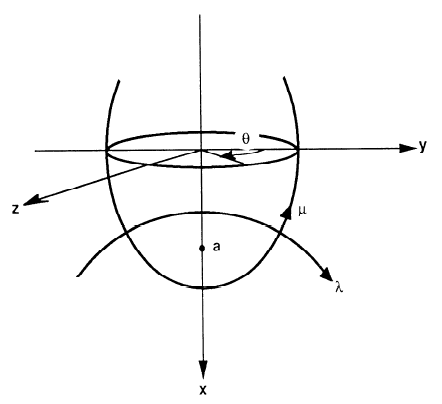
\includegraphics[scale=0.5]{prolate_spheroid_heart.png}
		\begin{tikzpicture}[scale=1]
			 \coordinate (a) at (0,-1);
  			\coordinate (b) at (0,1);
  			\node[label=below right:${}$] (a1) at (0,-1) {$\bullet$};
  			\node[label=above left:${}$] (b1) at (0,1) {$\bullet$};
  			
  			\node[label=below right:${a}$] (a1) at (-0.1,-0.9) {${}$};
  			\node[label=above left:${-a}$] (b1) at (0.2,0.9) {${}$};
  			
  			\ellipsebyfoci{draw}{a}{b}{1.6};
  			\ellipsebyfoci{draw}{a}{b}{1};
  			\ellipsebyfoci{draw}{a}{b}{3};
  			\pgfmathsetmacro{\e}{1}   % eccentricity
    		\pgfmathsetmacro{\a}{0.8}
    		\pgfmathsetmacro{\b}{(\a*sqrt((\e)^2/(\a)^2-1)} 
    		\draw plot[domain=-2:2] ({\b*sinh(\x)},{\a*cosh(\x)});
    		\draw plot[domain=-2:2] ({\b*sinh(\x)},{-\a*cosh(\x)});
    		
    		\pgfmathsetmacro{\c}{1}   % eccentricity
    		\pgfmathsetmacro{\d}{0.3}
    		\pgfmathsetmacro{\f}{(\d*sqrt((\c)^2/(\d)^2-1)} 
    		\draw plot[domain=-2:2] ({\f*sinh(\x)},{\d*cosh(\x)});
    		\draw plot[domain=-2:2] ({\f*sinh(\x)},{-\d*cosh(\x)});
    		
			\node[label=below:$\mu_1$] (mu1) at (2.5,3.5) {};
    		\node[label=below:$\mu_2$] (mu2) at (3.7,1.5) {};
    		\node[label=below:${\mu_3}$] (mu3) at (3.7,-0.8) {};
    		\node[label=below:${\mu_4 }$] (mu4) at (2.5,-2.8) {};
    		\node[label=below right:${\mu_5=\pi}$] (mu0) at (-0.3,-3.6) {};
    		\node[label=above right:${\mu_0=0}$] (mu0) at (-0.3,3.8) {};
    		\node[font=\tiny,scale=1] (lambda0) at (-0.25,0) {${\lambda_0}$};
    		\node[font=\footnotesize,scale=1] (lambda1) at (-1.43,0) {${\lambda_1}$};
    		\node[font=\normalsize,scale=1] (lambda2) at (-3.1,0) {${\lambda_2}$};
    		\pgfmathsetmacro{\cc}{1}   % eccentricity
    		\pgfmathsetmacro{\dd}{1}
    		\pgfmathsetmacro{\ff}{(\dd*sqrt((\cc)^2/(\dd)^2-1)} 
    		\draw[dashed] plot[domain=-2:2] ({\ff*sinh(\x)},{\dd*cosh(\x)});
    		\draw[dashed] plot[domain=-2:2] ({\ff*sinh(\x)},{-\dd*cosh(\x)});
		\end{tikzpicture}
		\caption{Elliptisches Koordinatensystem. Punkt wird beschrieben durch die Schnittstelle einer
		Hyperbel $\mu_i$ mit einer Ellipse $\lambda_i$, wobei diese konfokal sind, also die gleichen Brennpunkte
		 ($a$ und $-a$) besitzen.}
		\label{figure:elliptic_coordinates}
	\end{figure}
	\begin{figure}[h] % h for here, b for bottom, t for top position
		\centering % center the figure
		\begin{tikzpicture}[scale=1]
			 \coordinate (a) at (0,-1);
  			\coordinate (b) at (0,1);
  			\node[label=below right:${}$] (a1) at (0,-1) {$\bullet$};
  			\node[label=above left:${}$] (b1) at (0,1) {${}$};
  			
  			\node[label=below right:${a}$] (a1) at (-0.1,-0.9) {${}$};
  			
  			
  			
  			
  			\pgfmathsetmacro{\e}{1}   % eccentricity
    		\pgfmathsetmacro{\a}{0.4}
    		\pgfmathsetmacro{\b}{(\a*sqrt((\e)^2/(\a)^2-1)} 
    		
    		\draw[->] plot[domain=-1.8:2] ({{\b*sinh(\x)}},{-\a*cosh(\x)});
    		
    		\node[label=below:$x$] (x) at (0,-4) {};
    		\draw[->,dashed] (0,4) -- (x);
    		
    		\node[label=below:${\lambda}$] (mu3) at (3.7,-0.9) {};
    		\draw[ 
        decoration={markings, mark=at position 0.87 with {\arrow{>}}},
        postaction={decorate}
        ]
        (0,0) ellipse (2.25cm and 2.5cm);
    	
    	\draw[ 
        decoration={markings, mark=at position 0.9 with {\arrow{<}}},
        postaction={decorate}
        ]
        (0,0.25) ellipse (2.22cm and 0.3cm);
    		
    	
    	\node[label=right:$y$] (y) at (3.7,0.35) {};
    	\node[label=below:$z$] (z) at (-3.3,-1) {};
    	\draw[->,dashed] (0,0.25) -- (y);
    	\draw[->,dashed] (0,0.25) -- (z);
    	
    	
    	\node[label=right:$\mu$] (mu) at (1.3,-2){};
		\node[label=below right:$\theta$] (theta) at (1.2,0.1){};    	
    	
		\end{tikzpicture}
		
		
		
		\caption{ Darstellung eines <prolate spheroidal coordinate system> welches durch Rotation eines elliptischen
		Koordinatensystems um die $x$ - Achse entsteht. Anschaulich betrachtet: 
		Bei fixiertem $\mu$ und $\theta$ führt eine Änderung von $\lambda$
		zu einer Bewegung auf einer Hyperbel, bei fixiertem $\lambda$ und $\theta$ führt eine Änderung von
		$\mu$ zu einer Bewegung auf einer Ellipse und bei fixiertem $\lambda$ und $\mu$ führt eine Änderung
		von $\theta$ zu einer Kreisbewegung.}
		\label{figure:ps_heart}
	\end{figure}
	Verwenden eines solchen Koordinatensystem hat von Vorteil, dass es - vorausgesetzt günstige Brennpunkte
	wurden gewählt -  bereits annähernd die Form eines Herzens beschreit. Im Datensatz wurde hierfür
	der Brennpunkt auf  $35.25$ gesetzt.\\
	Zu beachten ist außerdem, dass die $x$ - Achse von oben nach unten läuft.
	\clearpage
	\subsection{Lokales Koordinatensystem}
		Elemente des Gitters werden durch eine Teilmenge der Knotenmenge definiert.
		Knoten, die einem Element angehören werden als lokale Knoten des Elements
		bezeichnet. Auf diesen lokalen Knoten wird nun ein lokales, orthonormales 
		Koordinatensystem erstellt, wobei jeder lokale Knoten an einem Eckpunkt
		eines Würfels mit Seitenlänge eins liegt.
		Die Raumrichtungen des lokalen Koordinatensystems werden mit $\xi_i$
		bezeichnet.
		Zur vereinfachten Darstellung wird dies zunächst in zwei 
		Raumdimensionen veranschaulicht.\\
		In \autoref{figure:local_element_coordinates} bilden jeweils vier Knoten
		ein Element, wobei jeder Knoten durch einen Kreis symbolisiert wird.\\
		Das Beispielelement besteht in diesem Fall aus den Knoten mit globalen
		 Inidizes aus der Indexmenge $\{a,b,c,d\}$. Unabhängig davon wird jedem
		 Knoten in der lokalen Knotenmenge ein Index aus der Menge $\{1,2,3,4\}$
		 zugewiesen.\\
		\begin{figure}[h]
		\begin{tikzpicture}
		\node[label=right:$x$] (x) at (4,0) {};
		\node[label=above:$y$] (y) at (0,4){};
		\node[label=left:${(a)}$] (g1) at (1,0.7) {$\circ$};
		\node[label=right:${(b)}$] (g2) at (3,0.3) {$\circ$};
		\node[label=left:${(c)}$] (g3) at (1.45,2.9) {$\circ$};
		\node[label=above:${(d)}$] (g4) at (3.75,3.5) {$\circ$};
		\node[red] (gint) at (2.6,3.18) {$\bullet$};
		\draw[->] (0,0) -- (x);
		\draw[->] (0,0) -- (y);		
		\draw[dashed] (g2) -- (g4);
		\draw[dashed] (g3) -- (g4);
		\draw[dashed] (g1) -- (g2);
		\draw[dashed] (g3) -- (g1);
		\node[label=above right:${(2)}$] at (11,0) {};
		\node[label=above right:${(3)}$]  at (8,3) {};
		\node[label=above right:${(1)}$]  at (8,0) {};
		\node[label=right:$\xi_1$] (x1) at (12,0) {};
		\node[label=above :$\xi_2$] (x2) at (8,4) {};
		\node[label=left:${0}$] (l1) at (8,0) {$\circ$};
		\node[label=below:${1}$] (l2) at (11,0) {$\circ$};
		\node[label=left:${1}$] (l3) at (8,3) {$\circ$};
		\node[label=above right:$(4)$] (l4) at (11,3) {$\circ$};
		\node[red] (lint) at (9.5,3) {$\bullet$};
		\draw[->] (8,0) -- (x1);
		\draw[->] (8,0) -- (x2);
		\draw[dashed] (l2) -- (l4);
		\draw[dashed] (l3) -- (l4);
		
		\draw[->] (5,2) -- (6,2);
		\end{tikzpicture}
		\caption{Darstellung eines viereckigen Elements in globalen
		 $(x,y)$-Koordinaten (links) und die Abbildung auf die lokalen 
		 Elementkoordinaten (rechts).}
		 \label{figure:local_element_coordinates}
		\end{figure}\\		 
		Benachbarte Elemente im Gitter teilen sich die Knoten, über die sie in
	 	Kontakt stehen (siehe \autoref{figure:shared_nodes}). Somit teilen sich
	 	die Elemente an diesen Stellen auch die gleichen in den Knoten definierten
	 	Parameter, falls vorhanden.
	 	Um ein vorhandenes Gitter zu verfeinern müssen neue Knoten generiert
	 	werden. Dies kann Elementweise durch Interpolation der lokalen Knoten
	 	 erreicht werden. Dazu bietet es sich das lokale Koordinatensystem in 
	 	Verbindung mit geeigneten Basisfunktionen an. \\
	 	In drei Raumdimensionen funktioniert dies analog.
	 	\clearpage
		\begin{figure}[h]
		\begin{center}
		
		\begin{tikzpicture}
		\node[label=right:$x$] (x) at (8,0) {};
		\node[label=above:$y$] (y) at (0,4){};
		\node[blue] (g1) at (1,0.7) {$\bullet$};
		\node[green] (g2) at (3,0.3) {$\bullet$};
		\node[blue] (g3) at (1.45,2.9) {$\bullet$};
		\node[green] (g4) at (3.75,3.5) {$\bullet$};
		
		\draw[->] (0,0) -- (x);
		\draw[->] (0,0) -- (y);		
		\draw[dashed] (g2) -- (g4);
		\draw[dashed] (g3) -- (g4);
		\draw[dashed] (g1) -- (g2);
		\draw[dashed] (g3) -- (g1);
		\node[yellow] (g5) at (5,3) {$\bullet$};
		\node[yellow] (g6) at (5.5,1) {$\bullet$};
		\draw[dashed] (g4) -- (g5);
		\draw[dashed] (g2) -- (g6);
		\draw[dashed] (g5) -- (g6);
		\end{tikzpicture}
		\end{center}
		\caption{Zwei benachbarte Elemente. Die blauen Knoten gehören der lokalen 
		Knotenmenge von Element 1 an, die gelben Knoten der lokalen
		Knotenmenge von Element 2  und die grünen Knoten befinden sich in
		den lokalen Knotenmengen beider Elemente. }
		 \label{figure:shared_nodes}
		\end{figure}
		
		
		\begin{figure}[h]
		\begin{center}
		
		\begin{tikzpicture}
		\node[label=below left:$(1)$] (o) at (0,0) {};
		\node[label=below left:$\xi_1$] (x1) at (4,-1){};
		\node[label=right:$\xi_2$] (x2) at (3.2,1.2){};
		\node[label=left:$\xi_3$] (x3) at (0,3){};
		\node[black] (1) at (0,0) {$\bullet$};
		\node[black, label=below:$(2)$] (2) at (2,-0.53) {$\bullet$};
		\node[black, label=below:$(3)$] (3) at (1.6,0.6) {$\bullet$};
		\node[black, label=below:$(4)$] (4) at (3.4,0.15) {$\bullet$};
		
		\node[black, label=left:$(5)$] (5) at (0,1.7) {$\bullet$};
		\node[black, label=above:$(6)$] (6) at (2,1.23) {$\bullet$};
		\node[black, label=above:$(7)$] (7) at (1.6,2.2) {$\bullet$};
		\node[black, label=above:$(8)$] (8) at (3.44,1.8) {$\bullet$};
		
		\draw[->] (o) -- (x1);
		\draw[->] (o) -- (x2);
		\draw[->] (o) -- (x3);
		
		\draw (3) -- (4);
		\draw (2) -- (4);
		
		\draw (5) -- (7);
		\draw (7) -- (8);
		
		\draw (6) -- (8);
		\draw (2) -- (4);
		
		\draw (5) -- (6);
		\draw (2) -- (6);
		
			\draw (3) -- (7);
		\draw (4) -- (8);
		\draw[decoration={brace,mirror,raise=5pt},decorate]
  (0,0) -- node[below=6pt] {$1$} (2,-0.53);
		\end{tikzpicture}
		\end{center}
		\caption{lokales Koordinatensystem in drei Raumrichtungen. 
		Angegeben sind die lokalen Knotenindizes.}
		 \label{figure:3d_cell_heart}
		\end{figure}
		\label{subsec:local_coordinates}
	 	\subsection{Interpolation}\label{subsec:interpolation}
	 	Das generieren neuer Knoten in einem Element kann durch Interpolation
	 	mit verschiedenen Basisfunktionen erreicht werden. Zunächst wird wieder der 
	 	zweidimensionale Fall betrachtet. Relativ einfach geht dies mit den
	 	linearen Lagrange Basisfunktionen $\Psi_i$. Diese sind in Abhängigkeit
	 	von den lokalen Koordinaten $0 \leq \xi_i \leq 1$ wie folgt definiert
	 	\cite[S.~52]{modelling}:
	 	\begin{equation}
	 	\label{eq:linear_lagrange_2d}
	 	\begin{split}
	 	\Psi_1 (\xi_1,\xi_2) &= (1-\xi_1)(1-\xi_2)\\
	 	\Psi_2 (\xi_1,\xi_2) &= \xi_1(1-\xi_2)\\
	 	\Psi_3 (\xi_1,\xi_2) &= (1-\xi_1)\xi_2\\
	 	\Psi_4 (\xi_1,\xi_2) &= \xi_1\xi_2
	 	\end{split}
	 	\end{equation}
	 	Sei nun $v$ ein neuer Knoten, der an irgendeinem Punkt $(\xi_1,\xi_2)$ im
	 	lokalen liegt. Für die in $v$ definierten Parameter $u(\xi_1,\xi_2)$, gilt
	 	anschließend:
	 	\begin{equation}
	 	\label{eq:nodal_parameter_linear_lagrange}
	 	u(\xi_1,\xi_2) = \Psi_1 (\xi_1,\xi_2)u^{(1)} + \Psi_2 (\xi_1,\xi_2)u^{(2)}
	 	+ \Psi_3 (\xi_1,\xi_2)u^{(3)} + \Psi_4 (\xi_1,\xi_2)u^{(4)}
	 	\end{equation}
	 	Wobei $u^{(i)}$ dem Knoten mit Index $i$ des lokalen Koordinatensystems
	 	als Parameter zugewiesen wurde.\\
	 	Aus \autoref{eq:linear_lagrange_2d} ist ersichtlich, dass für 
	 	$(\xi_1,\xi_2) \in (\{0,1\} \times \{0,1\})$ jeweils die Werte 
	 	$u^{(1)}, u^{(2)}, u^{(3)}$ und $u^{(4)}$ berechnet werden. Stetigkeit
	 	der Interpolation über die Elementgrenzen ist durch das Teilen der 
	 	Kontaktknoten zweier Elemente gegeben.\\
	 	Eine Einschränkung der linearen Lagrange Interpolation ist die 
	 	Differenzierbarkeit. Bei dem Übergang von einem Element zum nächsten
	 	ist zwar der Wert der Parameter im geteilten Knoten identisch und
	 	somit stetig, dies muss jedoch nicht für die Ableitung gelten.\\
	 	Dies ist anschaulich im eindimensionalen Fall zu erkennen. 
	 	\autoref{figure:1d_linear_lagrange}		
	 	\begin{figure}[h]
	 	\begin{center} \begin{tikzpicture}
	 	\node[label=below:$\text{Element }1$] at (2,4){};
	 	\node[label=below:$\text{Element }2$] at (6,4){};
	 	\node[label=right:$x$] (x) at (8,0) {};
		\node[label=left:$u(x)$] (y) at (0,4){};
	 	\draw[->] (0,0) -- (x);
	 	\draw[->] (0,0) -- (y);
	 	\node[label=above right:$(i)$] (i) at (0,2){$\circ$};
	 	\node[label=below:$(i+1)$] (j) at (4,1){$\circ$};
	 	\node[label=above:$(i+2)$] (k) at (8,1.5){$\circ$};
	 	\draw[dashed] (i) -- (j);
	 	\draw[dashed] (j) -- (k);
	 	\draw[dotted] (4,0) -- (4,4);
	 	\end{tikzpicture}
	 	
	 	\end{center}
	 	\caption{Eindimensionale lineare Interpolation. Die gestrichelte Linie
	 	beschreibt eine lineare Lagrange Interpolation zwischen jeweils zwei
	 	 Punkten.}
	 	 \label{figure:1d_linear_lagrange}
	 	\end{figure}\\
	 	An der Grenze zwischen Element $1$ und Element $2$ in Knoten $i+1$ 
	 	hat die Funktion $u(x)$ einen Knick und ist somit nicht differenzierbar.
	 	\\ 
	 	Die Lagrange Basisfunktionen gehören somit zur Differentiationsklasse $C^0$
	 	\cite[S.~55]{modelling}. Es bietet sich an, Basisfunktionen zu
	 	wählen welche in $C^1$ liegen. Dies wird ermöglicht durch
	 	kubisch hermitesche Basisfunktionen. Zusätzlich zu den Parametern werden
	 	in jedem Knoten außerdem Ableitungen entsprechend der Raumrichtungen
	 	gesetzt. Da die Parameter in den Knoten benachbarter Elemente an den 
	 	Kontaktstellen übereinstimmen gilt dies natürlich auch für die
	 	Ableitungen. Im eindimensionalen Fall sind also zwei abhängige Variablen
	 	pro Knoten benötigt: $u, \frac{\partial u}{\partial \xi}$. In zwei
	 	Raumdimensionen schon vier: $u, \frac{\partial u}{\partial \xi_1},
	 	\frac{\partial u}{\partial \xi_2}, \frac{\partial^2 u}{\partial \xi_1 
	 	\xi_2}$. \cite[S.~58]{modelling}
	 	\\Die eindimensionalen kubisch hermitesche Basisfunktionen sind wie folgt definiert:
	 	\begin{equation}
	 	\begin{split}
	 	\mathrm{H}^0_1(\xi) &= 1 -3\xi^2 + 2\xi^3 \\
		\mathrm{H}^1_1(\xi) &= \xi(\xi-1)^2\\
		\mathrm{H}^0_2(\xi) &= \xi^2(3-2\xi)\\
		\mathrm{H}^1_2(\xi) &= \xi^2(\xi-1)
	 	\end{split}
	 	\label{eq:1d_hermite_polynom}
	 	\end{equation}
	 	Aus den in \autoref{eq:1d_hermite_polynom} gegebenen kubischen Polynomen lässt
	 	sich folgende Abhängigkeit des Parameters $u$ in zwei Raumdimensionen definieren\cite{paper2}:
	 	
	 	\begin{equation}
	 	\begin{split}
		u(\xi_1, \xi_2) &= \mathrm{H}^0_1(\xi_1)\mathrm{H}^0_1(\xi_2)u^{(1)}+
		 \mathrm{H}^0_2(\xi_1)\mathrm{H}^0_1(\xi_2)u^{(2)}\\
						&+ \mathrm{H}^0_1(\xi_1)\mathrm{H}^0_2(\xi_2)u^{(3)}+
		 \mathrm{H}^0_2(\xi_1)\mathrm{H}^0_2(\xi_2)u^{(4)}\\
		 &+\mathrm{H}^1_1(\xi_1) \mathrm{H}^0_1(\xi_2)
		 \left(\frac{\partial u}{\partial \xi_1}\right)^{(1)}
		 +\mathrm{H}^1_2(\xi_1) \mathrm{H}^0_1(\xi_2)
		 \left( \frac{\partial u}{\partial \xi_1}\right)^{(2)}\\
		 &+\mathrm{H}^1_1(\xi_1) \mathrm{H}^0_2(\xi_2)
		 \left(\frac{\partial u}{\partial \xi_1}\right)^{(3)}
		 +\mathrm{H}^1_2(\xi_1) \mathrm{H}^0_2(\xi_2)
		 \left( \frac{\partial u}{\partial \xi_1}\right)^{(4)}\\
		 &+\mathrm{H}^0_1(\xi_1) \mathrm{H}^1_1(\xi_2)
		 \left(\frac{\partial u}{\partial \xi_2}\right)^{(1)}
		 +\mathrm{H}^0_2(\xi_1) \mathrm{H}^1_1(\xi_2)
		 \left( \frac{\partial u}{\partial \xi_2}\right)^{(2)}\\
		 		 &+\mathrm{H}^0_1(\xi_1) \mathrm{H}^1_2(\xi_2)
		 \left(\frac{\partial u}{\partial \xi_2}\right)^{(3)}
		 +\mathrm{H}^0_2(\xi_1) \mathrm{H}^1_2(\xi_2)
		 \left( \frac{\partial u}{\partial \xi_2}\right)^{(4)}\\
		 		 &+\mathrm{H}^1_1(\xi_1) \mathrm{H}^1_1(\xi_2)
		 \left(\frac{\partial^2 u}{\partial \xi_1 \partial \xi_2}\right)^{(1)}
		 +\mathrm{H}^1_2(\xi_1) \mathrm{H}^1_1(\xi_2)
		 \left( \frac{\partial^2 u}{\partial \xi_1 \partial \xi_2}\right)^{(2)}\\
		  	&+\mathrm{H}^1_1(\xi_1) \mathrm{H}^1_2(\xi_2)
		 \left(\frac{\partial^2 u}{\partial \xi_1 \partial \xi_2}\right)^{(3)}
		 +\mathrm{H}^1_2(\xi_1) \mathrm{H}^1_2(\xi_2)
		 \left( \frac{\partial^2 u}{\partial \xi_1 \partial \xi_2}\right)^{(4)}\\
	 	\end{split}
	 	\label{eq:bicubic_hermite_iterpolation}
	 	\end{equation}
	 	Für die Interpolation im Herzmodell wird eine Kombination der obigen Verfahren benutzt um eine  
	 	dreidimensionale Interpolation in den einzelnen Elementen zu ermöglichen.\\
	 	Die Winkel $\theta$ und $\mu$ werden jeweils in alle drei Raumrichtungen mit linearen Lagrange
	 	Basisfunktionen interpoliert. $\lambda$ hingegen wird in $\xi_1$- und $\xi_2$- Richtung mit kubisch
	 	hermiteschen Basisfunktionen und in $\xi_3$-Richtung linear interpoliert. \\
	 	Da angenommen wird (TODO:REFERENZ), dass die Muskelfasern in der $(\xi_1,\xi_2)$ Ebene liegen, 
	 	wird beim Faserwinkel $\eta$ in $\xi_1$- und $\xi_2$-Richtung linear-
	 	 und in $\xi_3$ -Richtung kubisch hermitesch interpoliert\cite{paper2}.
	 	 
	\chapter{Das Herzmodell}
	\section{Geometrie}
		Um auf der Geometrie des Herzens bekannte Gleichungen zu lösen empfiehlt
		es sich die Geometrie in diskrete Teilgebiete (Elemente) aufzuteilen. 
		In diesem Fall wurden die einzelnen Elemente durch einen 
		Fitting-Prozess auf Basis von experimentell ermittelten dreidimensionalen
		Punkten erstellt.\cite{paper1} \\
		Im Datensatz enthalten sind die Koordinaten von 99 Knoten, welche 60 Elemente in Form von
		Hexaedern bilden. Bei den "Hexaedern" am Fuß des Herzens handelt es sich im Datensatz zwar um
		Hexaeder, jedoch bilden dort in Form eines \emph{Edge-Collapse} mehrere lokale Knoten auf den selben
		globalen Knoten ab, sodass die Form eines Prismas entseht (siehe \autoref{figure:edge_collapse}).
		ProMesh unterstützt dieses Feature jedoch nicht, also wurden diese Elemente direkt als Prisma 
		implementiert. 
		
		 In jedem Knoten eines Elements sind
		 Ableitungen entsprechend den lokalen Koordinaten 
		 (siehe \autoref{subsec:interpolation})
		gegeben, sodass eine neuer Knoten gegebenenfalls auch durch kubische hermitesche Interpolation
		erzeugt werden kann. Dies wird im Folgenden auch verwendet, um feinere
		Gitter aus dem Datensatz zu generieren.\\
		Da ein Knoten jeweils zu mehreren aneinandergrenzenden Elementen gehören
		kann, ist eine stetige Differenzierbarkeit über die einzelnen
		Elemente gegeben. \\
		Wichtig für die Modellierung des Herzens sind außerdem die Ausrichtungen
		der Muskelfasern, da diese letztendlich die elektrische Leitfähigkeit
		der Herzmuskulatur mitbestimmen. In jedem Knoten ist hierfür der Winkel der
		in diesem Punkte verlaufenden Muskelfasern zwischen den lokalen
		 Koordinatenachsen $\xi_1$ und $\xi_2$ angegeben (siehe \autoref{figure:fiver_angle}). 
		 Die Faserwinkel für neu erstellte Knoten
		 werden ebenfalls durch Interpolation aus den Faserwinkeln der benachbarten Knoten berechnet.
		 \clearpage
	\begin{figure}[h]
	\centering
	\begin{tikzpicture}
	\node[label=below left:$(1)$] (o) at (0,0) {};
		\node[label=below left:$\xi_1$] (x1) at (4,-1){};
		\node[label=right:$\xi_2$] (x2) at (3.2,1.2){};
		\node[label=left:$\xi_3$] (x3) at (0,3){};
		\node[blue] (1) at (0,0) {$\bullet$};
		\node[blue, label=below:$(2)$] (2) at (2,-0.53) {$\bullet$};
		\node[black, label=below:$(3)$] (3) at (1.6,0.6) {$\circ$};
		\node[black, label=below:$(4)$] (4) at (3.4,0.15) {$\circ$};
		
		\node[red, label=left:$(5)$] (5) at (0,1.7) {$\bullet$};
		\node[red, label=above:$(6)$] (6) at (2,1.23) {$\bullet$};
		\node[black, label=above:$(7)$] (7) at (1.6,2.2) {$\circ$};
		\node[black, label=above:$(8)$] (8) at (3.44,1.8) {$\circ$};
		
		\draw[dashed] (o) -- (2);
		\draw[->] (o) -- (x2);
		\draw[->] (o) -- (x3);
		\draw[->] (2) -- (x1);
		\draw (3) -- (4);
		\draw (2) -- (4);
		
		\draw (5) -- (7);
		\draw (7) -- (8);
		
		\draw (6) -- (8);
		\draw (2) -- (4);
		
		\draw[dashed] (5) -- (6);
		\draw (2) -- (6);
		
			\draw (3) -- (7);
		\draw (4) -- (8);
		
  		\draw[->] (5,1)--(6,1);
  		
  		\node[label=below left:$x$] (x11) at (11,-1){};
		\node[label=right:$y$] (x22) at (10.2,1.2){};
		\node[label=left:$z$] (x33) at (7,3){};
		
				
		\node[blue, label=below:$(2)$] (22) at (1+7,-0.2) {$\bullet$};
		\node[black, label=below:$(3)$] (33) at (1.6+7,0.6) {$\circ$};
		\node[black, label=below:$(4)$] (44) at (3.4+7,0.15) {$\circ$};
		
		
		\node[red, label=left:$(6)$] (66) at (1+7,1.3) {$\bullet$};
		\node[black, label=above:$(7)$] (77) at (1.6+7,2.2) {$\circ$};
		\node[black, label=above:$(8)$] (88) at (3.44+7,1.8) {$\circ$};
		
		 \draw[->] (7,0) -- (x11);
		 \draw[->] (7,0) -- (x22);
		 \draw[->] (7,0) -- (x33);
		 \draw (88) -- (66);
		 \draw (77) -- (33);
		 \draw (33) -- (44);
		\draw (22) -- (44);
		\draw (66)-- (22);
		\draw (66) -- (77);
		\draw (77) -- (88);
		\draw (33) -- (22);
		\draw (44) -- (88);
		
		 
	\end{tikzpicture}
	\caption{Beispiel für einen \emph{Edge Collapse}: jeweils zwei farblich markierte Knoten im lokalen 
	Koordinatensystem bilden auf denselben globalen Knoten ab. Es ergibt sich dir Form eines Prismas.}
	\label{figure:edge_collapse}
	\end{figure}
	\begin{figure}[h!] % h for here, b for bottom, t for top position
		\centering % center the figure
		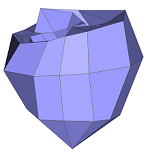
\includegraphics{heart000.png}
		\caption{Darstellung der Herzgeometrie mit 99 Knoten in ProMesh}
		\label{figure:heart000}
	\end{figure}
		\begin{figure}[h!] % h for here, b for bottom, t for top position
		\centering % center the figure
		\begin{tikzpicture}
			\node[label=above:$\xi_3$] (xi3) at (-1.1,-1.5){};
			\node[label=below:$\xi_1$] (xi1) at (3,0) {};
			\node[label=left:$\xi_2$] (xi2) at (0,3) {};
			\node[label=above:$f$] (f) at (2,1) {};
			\draw[->] (0,0) -- (xi1);
			\draw[->] (0,0) -- (f);
			\draw[->] (0,0) -- (xi2);
			\draw[->, dashed] (0,0) -- (xi3); 
			\node[label=right:$\eta$] (eta) at (1, 0.225) {};
			\draw (1,0) to[bend right=70] (0.9, 0.45);
		\end{tikzpicture}
		\caption{Faserwinkel $\eta$, angegeben in lokalen Koordinaten, wobei angenommen wird dass dieser in der
		 $(\xi_1,\xi_2)$- 
		Ebene liegt.}
		\label{figure:fiver_angle}
	\end{figure}
	\section{EX File Format und OpenCMISS Zinc}
	Der Datensatz besteht aus jeweils einer $\verb!heart.exnode!$ und $\verb!heart.exelem!$ Datei.\\
	 In 
	$\verb!heart.exnode!$ 
	sind 99 Knoten mit den räumlichen Koordinaten (in <prolate spheroidal coordinates>) sowie den Faserwinkeln
	gegeben. Falls ein Wert durch Polynome höheren Grades interpoliert wird, sind außerdem die jeweils benötigten
	Ableitungen des Werts bezüglich der lokalen Koordinaten gespeichert.  \\
	$\verb!heart.exelem!$ beschreibt die einzelnen Elemente des Modells, also welche Knoten zu welchen Elementen
	gehören und welche Basisfunktionen zur Interpolation neuer Knoten verwendet werden. Genaueres zum 
	sogenannten \verb!EX File Format! unter \cite{exfile}. \\\\
	Die Daten können mit der \verb!OpenCMISS-Zinc! API gelesen und bearbeitet werden. Diese stellt unter Anderem
	Anbindungen für Python und C++ bereit, welche für diese Arbeit verwendet wurden (Version 1.3.0.20180409141131
	der Linux Development-Distribution; Download und Hinweise zur Installation unter 
	\cite{opencmiss-zinc-getting-started}).
		\\	
	Um mit der Zinc- Bibliothek zu arbeiten muss
	 zunächst ein \verb!Context! Objekt erstellt werden, welches das einzige Objekt
	der Bibliothek ist das von keiner Methode eines anderen Objekts erstellt wird. Daraus folgt auch, dass
	jedes andere benötigte Objekt direkt oder indirekt von diesem  erstellt wird. Ein \verb!Region! Objekt
	wird beispielsweise direkt über \verb!Context.getDefaultRegion()! erstellt und ermöglicht es eine
	Datei des EX File-Formats einzulesen. Die wichtigsten Objekte der Zinc Bibliothek und wofür diese verwendet 
	 wurden werden nun
	kurz angeschnitten:
	
	\begin{description}
		\item[Context]\hfill \\
		Wie schon oben erwähnt muss in jedem Fall ein \verb!Context! erstellt werden, um mit der Zinc- Bibliothek
		erbeiten zu können.\\
		\item[Region]\hfill \\ 
		Kann als Analogon einer Ordnerhierarchie angesehen werden. Falls dem Benutzer eine Region ausreicht,
		kann vom Context eine standard-Region erstellt werden, was auch verwendet wurde. Die Region vermag es
		außerdem, Dateien vom EX-File Format zu lesen und zu schreiben.
		\item[Fieldmodule]\hfill \\ 
		Erstellt von \verb!Region! . Dieses Objekt ist hauptsächlich dazu da, Objekte vom Typ \verb!Field!
		zu verwalten. Wird verwendet um einen Großteil der verwendeten Objekte zu erzeugen. 
		\item[Fieldcache]\hfill \\ 
		Erstellt von \verb!Fieldmodule!. Im Fieldcache können Orte zur späteren Auswertung gespeichert werden.
		Dieser Ort kann beispielsweise ein Element inklusive lokalen \\$\xi_i$-Koordinaten oder ein Knoten sein.
		\item[Mesh/Nodeset]\hfill \\ 
		Erstellt von \verb!Fieldmodule!. Ein Mesh beschreibt eine Menge an Elementen, wobei jedem Element ein
		 Index zugeordnet ist. Besitzt Funktionen um Elemente zu erstellen oder zu löschen.\\
		 Nodeset verhält sich ähnlich, nur dass es sich, wie der Name bereits vermuten lässt, um eine Menge
		 von Knoten handelt. 
		\item[Field]\hfill \\ 
		Erstellt von \verb!Fieldmodule!. Speichert die Werte der Parameter an den Knoten/Elementen. Soll 
		beispielsweise ein Parameter eines Knotens ausgegeben werden, muss dieser Knoten im Fieldcache als Ort
		gespeichert werden, woraufhin das Feld an der im Fieldcache spezifizierten Stelle abgefragt wird.
		
\end{description}
	Eine Dokumentation der Zinc-API ist hier zu finden:\cite{opencmiss-zinc-api}
	\clearpage
	
	\chapter{Praktischer Teil}
	\section{Generieren feiner Gitter}
	Offensichtlicher Weise ist ProMesh nicht in der Lage, Dateien des EX-File Formats zu lesen. Am Ende
	 muss also zur Visualisierung eine Umwandlung in ein von ProMesh lesbares Format geschehen. In diesem Fall
	 wurde das \emph{Visualisation Toolkit}, kurz VTK verwendet. Dieses bietet die Möglichkeit ein 
	 unstrukturiertes Gitter in XML-Format mit der Endung \verb!.vtu! abzuspeichern. Dafür wurde ein 
	 Konverter geschrieben, der die erstellten Gitter in eine \verb!.vtu!- Datei übersetzt welche anschließend
	 von ProMesh gelesen werden kann.\\\\
	 Zuständig für das Erstellen feinerer Gitter ist die das Klasse \verb!mesh_generator!. Diese bietet die 
	 Möglichkeit über verschiedene \verb!set!- Funktionen die Anzahl der Verfeinerungen in die drei Raumrichtungen
	 für das Herz und die Muskelfasern zu bestimmen, sowie die Namen der verwendeten Dateien zu ändern.
	  \\Der \verb!mesh_generator.set_refinement(v,h,r)! Befehl
	 nimmt drei Integer $\geq$ 0 entgegen, und setzt die Verfeinerung auf $v$- mal in vertikale Richtung,
	  $h$- mal in
	 horizontale Richtung und $r$- mal in radiale Richtung. \\(Analoges gilt für die 
	 \verb! mesh_generator.set_refinement_fibers(v,h,r))! -Funktion.)\\
	 Die Verfeinerung beruht auf dem Prinzip, dass aus einem gegebenen Element neue Knoten über Interpolation
	 generiert werden, welche wiederum neue Elemente bilden. Da jedes Element auf ein lokales, orthonormales
	 Koordinatensystem abbildet, bei dem die jeweiligen Eckpunkte eines Würfels mit Kantenlänge $1$ die Knoten
	 des Elements darstellen (vergleiche \autoref{subsec:local_coordinates}), kann die Verfeinerung auf
	 diesem lokalen Koordinatensystem stattfinden. Anschließend muss lediglich eine Rücktransformation auf die
	 globalen Koordinaten stattfinden. Dies ist in zwei Dimensionen anschaulich in
	 \autoref{figure:interpolation_2d_local_coords} dargestellt. Dort findet in beide Raumrichtungen eine
	 einfache Verfeinerung statt.  Aus einem Element werden also vier neue Elemente generiert. Grundsätzlich ist
	 es so, dass jede Verfeinerungsstufe in eine Raumrichtung die Anzahl der Elemente in dieser Raumrichtung 
	 verdoppelt. Im dreidimensionalen Fall des Herzens nimmt also die Anzahl der Elemente mit Faktor
	 $2^{(v + h + r)}$ zu, wobei $v$, $h$ und $r$ die Anzahl der Verfeinerungen in die Raumrichtungen sind.
	 Da zu Beginn 60 Elemente existieren, gilt für die Gesamtanzahl an Elementen nach der Verfeinerung:\[
	 	\#\text{Elemente }= 60\cdot 2^{(v + h + r)}\]
	 \clearpage
	 
	 \begin{figure}[h]
	 \begin{tikzpicture}
	 %Element 1
	 \node[label=below:$x$] (x1) at (3,0) {};
	 \node[label=left:$y$] (y1) at (0,3) {};
	 \draw[->] (0,0) -- (x1);
	 \draw[->] (0,0) -- (y1);
	 \node[label=below:${}$] (a) at (1,2.5) {$\bullet$};
	 \node[label=below:${}$] (b) at (0.5,0.5) {$\bullet$};
	 \node[label=below:${}$] (c) at (3,2.5) {$\bullet$};
	 \node[label=below:${}$] (d) at (2.5,0.5) {$\bullet$};
	 
	 \draw (a) to [out=230, in=100](b);
	 \draw (a) to (c);
	 \draw (c) to [out=230, in=100](d);
	 \draw (b) to (d);
	 \draw[->] (3,1.5) -- (3.5,1.5);
	 
	 \node[label=below:$\xi_1$] (xi11) at (7,0) {};
	 \node[label=left:$\xi_2$] (xi21) at (4,3) {};
	 \draw[->] (4,0) -- (xi11);
	 \draw[->] (4,0) -- (xi21);
	 \node[label=below:${}$] (11) at (4,0) {$\bullet$};
	 \node[label=below:${}$] (21) at (6,0) {$\bullet$};
	 \node[label=below:${}$] (31) at (4,2) {$\bullet$};
	 \node[label=below:${}$] (41) at (6,2) {$\bullet$};
	 
	 \draw (21) to (41);
	 \draw (41) to (31);
	 
	 \draw[->] (7,1.5) -- (7.5,1.5);
	 
	  \node[label=below:$\xi_1$] (xi12) at (11,0) {};
	 \node[label=left:$\xi_2$] (xi22) at (8,3) {};
	 \draw[->] (8,0) -- (xi12);
	 \draw[->] (8,0) -- (xi22);
	 \node[label=below:${}$] (12) at (8,0) {$\bullet$};
	 \node[label=below:${}$] (22) at (10,0) {$\bullet$};
	 \node[label=below:${}$] (32) at (8,2) {$\bullet$};
	 \node[label=below:${}$] (42) at (10,2) {$\bullet$};
	 
	 \draw (22) to (42);
	 \draw (42) to (32);
	 
	 \node[red,label=below:${}$] (i1) at (8+1,0) {$\bullet$};
	 \node[red,label=below:${}$] (i2) at (10,1) {$\bullet$};
	 \node[red,label=below:${}$] (i3) at (8+1,2) {$\bullet$};
	 \node[red,label=below:${}$] (i4) at (10-2,2-1) {$\bullet$};
	 \node[red,label=below:${}$] (i5) at (10-1,2-1) {$\bullet$};
	 
	 \draw[dashed] (i1) to (i3);
	 \draw[dashed] (i4) to (i2);
	 
	 \draw[->] (11,1.5) to (11.5,1.5);
	 
	 \node[label=below:$x$] (x2) at (15,0) {};
	 \node[label=left:$y$] (y2) at (12,3) {};
	 \draw[->] (12,0) -- (x2);
	 \draw[->] (12,0) -- (y2);
	 \node[label=below:${}$] (a1) at (13,2.5) {$\bullet$};
	 \node[label=below:${}$] (b1) at (12.5,0.5) {$\bullet$};
	 \node[label=below:${}$] (c1) at (15,2.5) {$\bullet$};
	 \node[label=below:${}$] (d1) at (14.5,0.5) {$\bullet$};
	 
	 \draw (a1) to [out=230, in=100](b1);
	 \draw (a1) to (c1);
	 \draw (c1) to [out=230, in=100](d1);
	 \draw (b1) to (d1);
	 
	 \node[red,label=below:${}$] (ii1) at (14,2.5) {$\bullet$};
	 \node[red,label=below:${}$] (ii2) at (13.5,0.5) {$\bullet$};
	 \node[red,label=below:${}$] (ii3) at (12.45,1.6) {$\bullet$};
	 \node[red,label=below:${}$] (ii4) at (14.45,1.6) {$\bullet$};
	 \node[red,label=below:${}$] (ii5) at (13.45,1.6) {$\bullet$};
	 
	 \draw[dashed] (ii1) to [out=230, in=100](ii2);
	 \draw[dashed] (ii3) to (ii4);
	 \end{tikzpicture}
	 \caption{Graphische Darstellung der Verfeinerung eines verzerrten Elements. Zunächst wird das Element in
	 lokalen Koordinaten umgewandelt, dort werden neue Knoten generiert (Als rote Punkte dargestellt).
	 Das Element wird mit den neuen Knoten zurück in globale Koordinaten transformiert. Zu erkennen ist, dass
	 die Elementgrenzen der neuen Elemente ebenfalls verzerrt sind.}
	 \label{figure:interpolation_2d_local_coords}
	 \end{figure}
	 Der Algorithmus zur Verfeinerung des Gitters iteriert über alle Elemente des Gitters und unterteilt jedes
	 Element gemäß der gewählten Verfeinerungsstufen in neue Elemente mit gegebenenfalls neuen Knoten. Unter 
	 Betrachtung von \autoref{figure:double_nodes} lässt sich feststellen, dass ein Knoten $v_i$ am Rand eines
	  Elements
	 die gleichen globalen Koordinaten wie ein bereits generierter Knoten $v_j$ am Rand
	  eines benachbarten Elements haben
	 kann. Da die Anforderung an die Stetigkeit über Elementgrenzen hinweg erfüllt ist, müssen $v_i$ und $v_j$
	 deshalb die gleichen Parameter haben, also gilt $u(v_i) = u(v_j)$ und es kann $v_j$ für $v_i$ verwendet 
	 werden.
	 
	
	\begin{figure}[h]
	\centering
	\begin{tikzpicture}
	 \node[label=below:$x$] (x1) at (6,0) {};
	 \node[label=left:$y$] (y1) at (0,3) {};
	 \draw[->] (0,0) -- (x1);
	 \draw[->] (0,0) -- (y1);
	

	 \node[label=below:${}$] (a1) at (13-12,2.5) {$\bullet$};
	 \node[label=below:${}$] (b1) at (12.5-12,0.5) {$\bullet$};
	 \node[label=below:${}$] (c1) at (15-12,2.5) {$\bullet$};
	 \node[label=below:${}$] (d1) at (14.5-12,0.5) {$\bullet$};
	 
	 \draw (a1) to [out=230, in=100](b1);
	 \draw (a1) to (c1);
	 \draw (c1) to [out=230, in=100](d1);
	 \draw (b1) to (d1);
	 
	 \node[label=below:${}$] (a2) at (13-10,2.5) {$\bullet$};
	 \node[label=below:${}$] (b2) at (12.5-10,0.5) {$\bullet$};
	 \node[label=below:${}$] (c2) at (15-10,2.5) {$\bullet$};
	 \node[label=below:${}$] (d2) at (14.5-10,0.5) {$\bullet$};
	 \node[red,label=below:${}$] (ii1) at (14-12,2.5) {$\bullet$};
	 \node[red,label=below:${}$] (ii2) at (13.5-12,0.5) {$\bullet$};
	 \node[red,label=below:${}$] (ii3) at (12.45-12,1.6) {$\bullet$};
	 \node[orange,label=below:${}$] (ii4) at (14.45-12,1.6) {$\bullet$};
	 \node[red,label=below:${}$] (ii5) at (13.45-12,1.6) {$\bullet$};
	 \node[blue,label=below:${}$] (ii6) at (14-10,2.5) {$\bullet$};
	 \node[blue,label=below:${}$] (ii7) at (13.5-10,0.5) {$\bullet$};
	 \node[black,label=below:${}$] (ii8) at (12.45-10,1.6) {$\bigcirc$};
	 \node[blue,label=below:${}$] (ii9) at (14.45-10,1.6) {$\bullet$};
	 \node[blue,label=below:${}$] (ii10) at (13.45-10,1.6) {$\bullet$};
	 
	 	 
	 \draw (a2) to [out=230, in=100](b2);
	 \draw (a2) to (c2);
	 \draw (c2) to [out=230, in=100](d2);
	 \draw (b2) to (d2);
	 	 \draw[dashed] (ii1) to [out=230, in=100](ii2);
	 \draw[dashed] (ii3) to (ii4);
	 \draw (a) to [out=230, in=100](b);
	 \draw (a) to (c);
	 \draw (c) to [out=230, in=100](d);
	 \draw (b) to (d);
	 	 \draw[dashed] (ii6) to [out=230, in=100](ii7);
	 \draw[dashed] (ii8) to (ii9);
	\end{tikzpicture}	
	\caption{Zwei benachbarte, verfeinerte Elemente. Zu beachten ist, dass der markierte Knoten beim 
	Bearbeiten beider Elemente entsteht, falls keine weiteren Vorkehrungen getroffen werden.}
	\label{figure:double_nodes}
	\end{figure}
	Die Herausforderung besteht nun darin, Knoten gleicher Position zu erkennen und anschließend zu verwenden.
	Ein naiver Ansatz wäre dafür jeden  potentiell zu erstellenden Knoten mit jedem bereits verwendeten Knoten
	zu vergleichen und erst wenn der Vergleich mit allen Knoten negativ war, diesen zu erstellen.
	Dies führt aber für große Knotenmengen zu nicht akzeptabler Rechenzeit.\clearpage
	
	
	Die verwendete Methode um doppelte Knoten zu vermeiden greift auf den naiven Ansatz zurück, führt diesen
	allerdings auf Knotenmengen aus, die durch ein vorsortieren sehr viel kleiner sind als.\\	
	Vor dem eigentlichen Verfeinern wird jedem Knoten $v_i$ ein Wert $w(v_i)$ zugeordnet, welcher der Summe seiner
	 $x,y$ und $z$
	Koordinaten entspricht. Daraufhin werden $10.000$ Behälter erstellt und jedem Behälter $B_j$ wird ein 
	gleichgroßes Intervall $I_j$
	zugeordnet, wobei das Minimum (Maximum) aller $w(v_i)$ im Intervall des ersten (letzten) Behälters liegt.\\
	Anschließend kann für alle Knoten bestimmt werden:
	Knoten $v_i$ ist genau dann Behälter $B_j$ zuzuordnen, wenn gilt: $w(v_i) \in I_j$.\\\\
	 Sei nun $v_{\text{neu}}$
	ein potentieller Knoten, mit $w(v_{\text{neu}}) \in I_j$. Es wird nun $v_{\text{neu}} $ mit allen Knoten
	 $v_i \in B_{j-1}\cup B_{j} \cup B_{j+1}$ verglichen. Sollte einer dieser Knoten mit $v_{\text{neu}}$
	 übereinstimmen, wird dieser Knoten verwendet. Andernfalls wird $v_{\text{neu}}$ erstellt und $B_j$
	  zugeordnet.\\	 
	 Für den Fall dass der Wert eines Knotens nahe einer Intervallgrenze eines Behälters liegt und 
	 Rundungsfehler nicht
	 ausgeschlossen werden können, wird  in der Vereinigung des Behälters mit seinen beiden benachbarten
	 Behältern gesucht.\\

	
	
	
	
	
	
	
	
	
	
	
	
	
	
	
	
	\iffalse\begin{verbatim}
	 #Fields=2
	 1) coordinates, coordinate, prolate spheroidal, focus=  0.3525E+02, #Components=3
   		lambda.  Value index= 1, #Derivatives= 3 (d/ds1,d/ds2,d2/ds1ds2)
   		mu.  Value index= 5, #Derivatives= 0  
   		theta.  Value index= 6, #Derivatives= 0  
 2) fibres, anatomical, fibre, #Components=3
   		fibre angle.  Value index= 7, #Derivatives= 1 (d/ds1)
   		imbrication angle.  Value index= 9, #Derivatives= 0  
   		sheet angle.  Value index=10, #Derivatives= 3 (d/ds1,d/ds2,d2/ds1ds2)
   		Node:            1
     	0.1159700000000000E+01   0.2370300000000000E-02   0.2432300000000000E-02   0.5232600000000000E-03
    	 0.2042035224833366E+01
     	0.6021385919380437E+01
      -0.1327305442849168E+01  -0.3011391091391016E-01
     	0.0000000000000000E+00
      -0.2525962666533833E+01  -0.3298672286269282E+00   0.5475272396431411E+00  -0.5190783728356336E-01
	\end{verbatim}
	\fi
	
	
	
	
	% Enable bibliography, put the bib-file in the \bibliography{...} 
	% Choose a style, check for instance apa, unsrt
	\printglossary[type=\acronymtype,title=List of Notation and Abbreviations]
	
	\bibliographystyle{unsrt}
	\bibliography{template_thesis}
\end{document}
